\documentclass{article}

% Encoding and fonts
\usepackage[T1]{fontenc}
\usepackage[utf8]{inputenc}
\usepackage{lmodern}
\usepackage{textcomp}

% Typography
\usepackage{microtype}
\sloppy

% Math and graphics
\usepackage{amsmath}
\usepackage{tikz}
\usetikzlibrary{automata, positioning, shapes.geometric, shadows}

% Layout and headers
\usepackage{fancyhdr}
\usepackage{extramarks}

% Algorithms (loaded once)
\usepackage[plain]{algorithm}

% Page geometry (manual)
\topmargin=-0.45in
\evensidemargin=0in
\oddsidemargin=0in
\textwidth=6.5in
\textheight=9.0in
\headsep=0.25in
\linespread{1.1}
\setlength\parindent{0pt}

% Project metadata
\newcommand{\hmwkDueDate}{9 de janeiro}
\newcommand{\hmwkClass}{Sistemas Distribuídos}
\newcommand{\hmwkAuthorName}{%
  \textbf{André Santos A106854}\\ %
  \textbf{Daniel Parente A107363}\\ %
  \textbf{Pedro Ferreira A107292}\\ %
  \textbf{Tiago Martins A106938}   %
}

% Header/Footer
\pagestyle{fancy}
%\lhead{\textbf{} \textbf{}}
%\rhead{\textbf{}}
\lfoot{\lastxmark}
\cfoot{\thepage}
\renewcommand\headrulewidth{0.4pt}
\renewcommand\footrulewidth{0.4pt}

% Title
\title{%
  \vspace{2in}
  \textmd{\textbf{\hmwkClass}}\\
  \normalsize\vspace{0.1in}\small{Prazo de Entrega a \hmwkDueDate}\\
  \vspace{0.1in}
  \vspace{3in}
}
\author{\hmwkAuthorName}

\begin{document}

\maketitle

\pagebreak

\section{Arquitetura do Sistema}

A arquitetura desenvolvida para este sistema distribuído baseia-se num modelo cliente-servidor, concebido para suportar elevada concorrência e processamento eficiente de pedidos. A comunicação entre os intervenientes é realizada através do protocolo TCP, garantindo a entrega fiável de mensagens. Para maximizar o débito e a capacidade de resposta, foi implementado um protocolo de aplicação personalizado que suporta multiplexagem de pedidos numa única ligação física, permitindo que múltiplas \textit{threads} do lado do cliente comuniquem simultaneamente com o servidor sem bloqueios desnecessários.

A secção seguinte detalha os componentes principais desta arquitetura, partindo do cliente, passando pelo protocolo de comunicação e finalizando no servidor.

\subsection{Cliente}

A biblioteca cliente, encapsulada na classe \texttt{ClientLib}, fornece uma interface de alto nível para a interação com o serviço de vendas. Esta classe foi desenhada para ser \textit{thread-safe}, permitindo que a aplicação cliente utilize múltiplas \textit{threads} para invocar operações (como \texttt{addEvent} ou \texttt{login}) concorrentemente sobre a mesma instância do cliente.

A gestão da concorrência e da comunicação de rede é delegada a dois componentes fundamentais: a \texttt{TaggedConnection} e o \texttt{Demultiplexer}.

\begin{itemize}
    \item \textbf{Gestão de Concorrência:} O cliente não bloqueia a ligação TCP inteira enquanto espera por uma resposta. Em vez disso, utiliza um mecanismo de multiplexagem que permite enviar múltiplos pedidos sem aguardar pelas respostas anteriores (pipelining), maximizando a utilização da largura de banda.
    \item \textbf{Abstração:} O \texttt{ClientLib} abstrai a complexidade da serialização e da rede, expondo métodos simples com argumentos tipados (e.g., \texttt{String}, \texttt{int}) e lançando exceções verificadas em caso de falha.
\end{itemize}

\subsection{Protocolo de Comunicação}

O protocolo define estritamente o formato das mensagens trocadas e o mecanismo de serialização. A comunicação é orientada a mensagens (frames), evitando os problemas comuns de leitura de fluxos de bytes contínuos.

\subsubsection{Formato da Mensagem}
Cada unidade de comunicação é denominada \texttt{Frame} e possui a seguinte estrutura binária:
\begin{enumerate}
    \item \textbf{Tag (4 bytes):} Um identificador único inteiro gerado pelo cliente para cada pedido. Este identificador permite associar inequivocamente uma resposta ao pedido original.
    \item \textbf{Type (1 byte):} Código que identifica o tipo de operação (e.g., \texttt{LOGIN=2}, \texttt{ADD\_EVENT=3}) ou o tipo de resposta (\texttt{RESPONSE\_OK=50}).
    \item \textbf{Length (4 bytes):} O tamanho em bytes do corpo da mensagem (\textit{payload}).
    \item \textbf{Payload (variável):} Os dados da mensagem serializados manualmente.
\end{enumerate}

\subsubsection{Serialização}
A serialização é realizada manualmente através da classe utilitária \texttt{Serialization}, recorrendo a \texttt{DataInputStream} e \texttt{DataOutputStream}.

Uma otimização notável ocorre na serialização de listas de eventos (\texttt{serializeEventList}). Para evitar a repetição de strings (nomes de produtos) em listas grande, foi implementada uma codificação baseada em dicionário: envia-se primeiro uma lista de produtos únicos e, seguidamente, os registos de vendas referenciam os produtos através de índices inteiros, reduzindo drasticamente o tamanho da mensagem em cenários de alta carga.

\subsubsection{Multiplexagem e Demultiplexagem}
O componente \texttt{Demultiplexer} é o coração da comunicação concorrente no lado do cliente. O seu funcionamento detalhado é o seguinte:

\begin{enumerate}
    \item \textbf{Envio (\texttt{send}):} Quando uma \textit{thread} deseja enviar um pedido:
    \begin{enumerate}
        \item Adquire um \textit{lock} exclusivo para gerar uma nova \texttt{tag} sequencial.
        \item Cria um objeto \texttt{FrameQueue} (que contém um \textit{lock} e uma variável de condição) e regista-o num mapa de pedidos pendentes (\texttt{pending}), associado à \texttt{tag}.
        \item Envia o \texttt{Frame} através da \texttt{TaggedConnection}.
        \item Bloqueia na variável de condição da sua \texttt{FrameQueue} específica, aguardando apenas pela sua resposta. Outras \textit{threads} podem continuar a enviar pedidos enquanto esta aguarda.
    \end{enumerate}

    \item \textbf{Receção (\texttt{receiverLoop}):} Uma \textit{thread} de fundo (\textit{receiver}) dedicada lê continuamente da \textit{socket}:
    \begin{enumerate}
        \item Lê o cabeçalho do \texttt{Frame} e determina a sua \texttt{tag}.
        \item Consulta o mapa \texttt{pending} para encontrar a \texttt{FrameQueue} correspondente.
        \item Coloca a resposta na fila e sinaliza a variável de condição, acordando a \textit{thread} original que aguardava.
        \item Remove a entrada do mapa.
    \end{enumerate}
\end{enumerate}

Este mecanismo permite que $N$ \textit{threads} partilhem uma única ligação física de forma eficiente e segura.

\subsection{Servidor}

O servidor implementa uma arquitetura concorrente de alto desempenho, desenhada para maximizar o débito (\textit{throughput}) de escrita e minimizar a latência de leitura, garantindo simultaneamente a persistência e consistência dos dados.

\subsubsection{Gestão de Ligações e Concorrência}
O servidor adopta um modelo \textit{Thread-per-Client} otimizado com \textit{Worker Pools}. As ligações TCP são aceites por uma \texttt{ServerSocket} e delegadas a instâncias de \texttt{ClientHandler}. Ao contrário de uma abordagem ingénua onde cada cliente bloqueia uma \textit{thread} do sistema operativo indefinidamente, o servidor utiliza um padrão de \textit{Work Stealing} simplificado onde as operações pesadas são submetidas a pools de execução, libertando a thread de I/O para processar outros pacotes.

\subsubsection{Camada de Armazenamento (\texttt{Repository})}
O coração do sistema é a classe \texttt{Repository}, que orquestra o acesso aos dados utilizando uma estratégia híbrida de memória e disco, protegida por um \texttt{ReentrantReadWriteLock} para permitir leituras paralelas massivas.

\paragraph{Estratégia de Cache e Evicção (LRU)}
Para gerir o compromisso entre memória RAM e acesso ao disco, o sistema implementa uma hierarquia de caches sofisticada em \texttt{DayCache}:
\begin{itemize}
    \item \textbf{Hot Data (LRU):} Os dias mais recentes ou frequentemente acedidos são mantidos em memória. A implementação recorre a um \texttt{LinkedHashMap} em modo \textit{access-order}, que serve como uma cache LRU (\textit{Least Recently Used}). Quando o limite de memória ($S$ dias) é atingido, o dia menos recentemente utilizado é automaticamente despejado da memória, libertando recursos.
    \item \textbf{Carregamento Transparente:} Se um cliente solicita dados de um dia antigo que já foi despejado, o \texttt{Repository} carrega-o transparentemente do disco (\texttt{EventReader}) sem que a camada de negócio tenha conhecimento da falha de cache (\textit{cache miss}).
\end{itemize}

\paragraph{Agregação Preguiçosa (\texttt{AggregationCache})}
O cálculo de estatísticas (e.g., volume de vendas, preço médio) sobre milhões de eventos é computacionalmente dispendioso. Para mitigar este custo, o \texttt{AggregationCache} utiliza uma estratégia \textit{Lazy Evaluation}:
\begin{enumerate}
    \item Quando um dia é concluído (\textit{frozen}), os seus dados tornam-se imutáveis.
    \item As estatísticas não são pré-calculadas imediatamente. Em vez disso, o sistema aguarda pela primeira consulta (\textit{Query}).
    \item No primeiro acesso, o sistema computa as estatísticas de todos os produtos desse dia numa única passagem (\texttt{streamEvents}) e armazena o resultado em cache.
    \item Consultas subsequentes são servidas em tempo constante $O(1)$ a partir da cache, eliminando leituras de disco repetidas.
\end{enumerate}

\paragraph{Persistência com Duplo Buffer (\texttt{EventWriter})}
A latência de escrita no disco é, por norma, ordens de grandeza superior à latência de rede. Para evitar que operações de \texttt{addEvent} bloqueiem o cliente, foi implementado um padrão de \textit{Double Buffering} no \texttt{EventWriter}:
\begin{itemize}
    \item As escritas dos clientes são depositadas instantaneamente num \textit{buffer} em memória (\texttt{ArrayDeque}), protegido por um \textit{lock} de curta duração.
    \item Uma \textit{thread} de escrita dedicada (\textit{Writer Thread}) acorda, troca o ponteiro do buffer ativo com um buffer de reserva (operação atómica) e procede à escrita em disco do lote (\textit{batch}) completo.
    \item Isto desacopla a latência do disco da latência percebida pelo cliente, permitindo picos de carga muito superiores à velocidade física do armazenamento.
\end{itemize}

\subsubsection{Notificações em Tempo Real (\textit{Observer Pattern})}
O requisito de notificações (vendas simultâneas e consecutivas) apresenta um desafio de concorrência: como bloquear um cliente à espera de um evento futuro sem bloquear uma \textit{thread} de processamento do servidor?

A solução implementada combina o padrão \textit{Observer} com \textit{Deferred Responses}:
\begin{enumerate}
    \item \textbf{Suspensão:} Quando chega um pedido de notificação, o \texttt{RequestDispatcher} não retorna uma \texttt{Frame} de resposta. Em vez disso, regista um \texttt{NotificationCallback} no componente \texttt{CurrentDayObserver} e retorna um objeto especial \texttt{DeferredResponse}.
    \item \textbf{Libertação:} A \textit{thread} que processou o pedido termina a sua execução imediatamente, ficando disponível para servir outros clientes. A conexão TCP do cliente permanece aberta, mas "silenciosa".
    \item \textbf{Monitorização:} O \texttt{CurrentDayObserver} intercepta todas as escritas no sistema. Mantém estruturas de dados otimizadas (Mapas de Listas) para verificar eficientemente se os critérios (Ex: P1 e P2 vendidos) foram satisfeitos.
    \item \textbf{Disparo Assíncrono:} Quando a condição é cumprida, o \textit{Observer} executa o \textit{callback}, que serializa a resposta e a envia diretamente para a \textit{socket} do cliente, completando o ciclo pedido-resposta de forma assíncrona.
\end{enumerate}

\subsection{Integração da Arquitetura}

A Figura~\ref{fig:arch_full} ilustra o fluxo de dados e a interação entre os componentes de armazenamento, cache e notificação.

\begin{figure}[h]
\centering
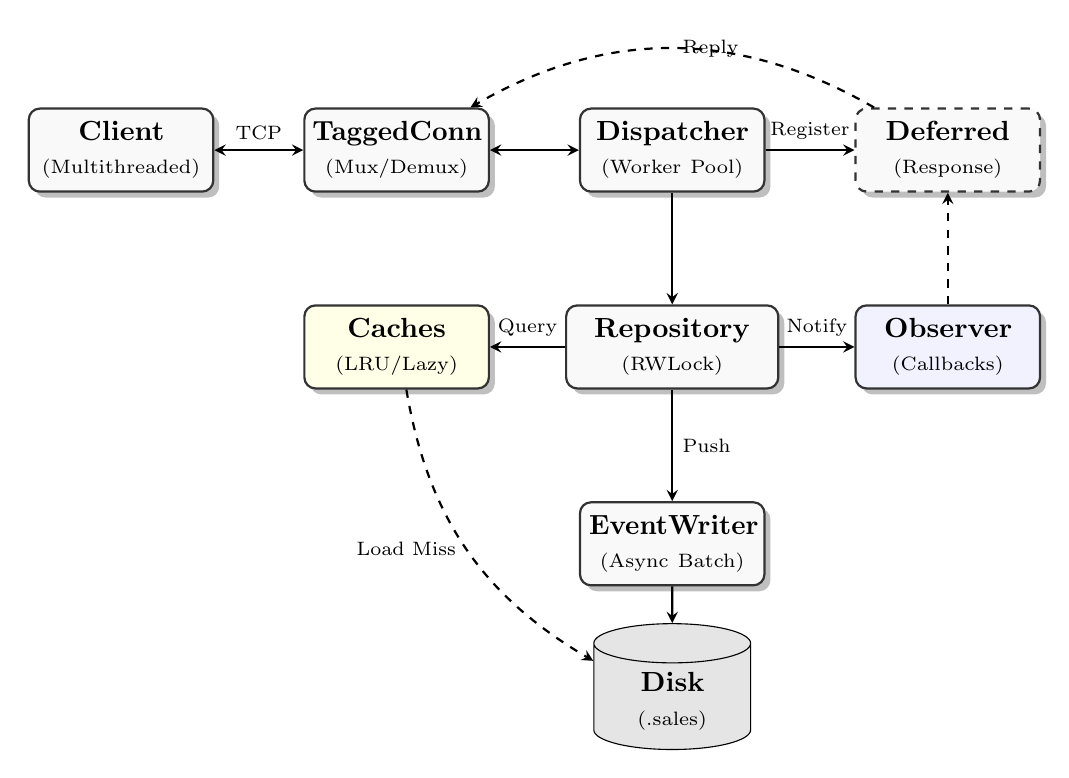
\begin{tikzpicture}[node distance=1.8cm, auto,
    component/.style={rectangle, draw=black!80, thick, fill=gray!5, text width=6em, text centered, rounded corners, minimum height=3em, drop shadow},
    thread/.style={circle, draw=black, fill=white, inner sep=2pt},
    store/.style={cylinder, draw=black, shape border rotate=90, aspect=0.25, fill=gray!20, text width=5em, align=center, minimum height=3em},
    arrow/.style={->, >=stealth, thick}
]

    % Client Side
    \node (client) [component] {\textbf{Client}\\\scriptsize(Multithreaded)};
    \node (conn) [component, right of=client, node distance=3.5cm] {\textbf{TaggedConn}\\\scriptsize(Mux/Demux)};

    % Server logic
    \node (dispatcher) [component, right of=conn, node distance=3.5cm] {\textbf{Dispatcher}\\\scriptsize(Worker Pool)};

    % Core Systems
    \node (repo) [component, below of=dispatcher, node distance=2.5cm, text width=7em] {\textbf{Repository}\\\scriptsize(RWLock)};

    % Notification Side
    \node (observer) [component, right of=repo, node distance=3.5cm, fill=blue!5] {\textbf{Observer}\\\scriptsize(Callbacks)};
    \node (deferred) [component, above of=observer, node distance=2.5cm, dashed] {\textbf{Deferred}\\\scriptsize(Response)};

    % Storage Side
    \node (writer) [component, below of=repo, node distance=2.5cm] {\textbf{EventWriter}\\\scriptsize(Async Batch)};
    \node (cache) [component, left of=repo, node distance=3.5cm, fill=yellow!10] {\textbf{Caches}\\\scriptsize(LRU/Lazy)};

    % Disk
    \node (disk) [store, below of=writer, node distance=2.0cm] {\textbf{Disk}\\\scriptsize(.sales)};

    % Connections
    \draw [arrow, <->] (client) -- node[above] {\scriptsize TCP} (conn);
    \draw [arrow, <->] (conn) -- (dispatcher);

    % Logic Flows
    \draw [arrow] (dispatcher) -- (repo);
    \draw [arrow] (dispatcher) -- node[above] {\scriptsize Register} (deferred);
    \draw [arrow, dashed, bend right] (deferred) to node[right] {\scriptsize Reply} (conn);
    \draw [arrow, dashed] (observer) -- (deferred);

    % Storage Flows
    \draw [arrow] (repo) -- node[right] {\scriptsize Push} (writer);
    \draw [arrow] (writer) -- (disk);
    \draw [arrow] (repo) -- node[above] {\scriptsize Query} (cache);
    \draw [arrow] (repo) -- node[above] {\scriptsize Notify} (observer);
    \draw [arrow, dashed, bend right=25] (cache) to node[left] {\scriptsize Load Miss} (disk);

\end{tikzpicture}
\caption{Arquitetura detalhada do Servidor: Integração de \textit{Caching}, Persistência Assíncrona e Notificações.}
\label{fig:arch_full}
\end{figure}

\end{document}